\section{Badania}

Przetestowano dwie konfiguracje agentów, wraz ze sposobami realizacja Q-learningu oraz metody przyznawania nagród (jeśli dotyczy).

Konfiguracje agentów:
\begin{itemize}
	\item Q-Learning - Random,
	\item Q-learning - Q-learning.
\end{itemize}

Typy uczenia Q-learningu:
\begin{itemize}
	\item step mode, z wykorzystaniem oceny stanów gry poprzez:
	\begin{itemize}
		\item nadawanie nagrody $\pm 1$ na końcu gry, a $0$ w jej trakcie,
		\item uczenie nadzorowane;
	\end{itemize}
	\item batch mode.
\end{itemize}

Dodatkowo zbadano wpływ parametrów $\alpha, \gamma, \epsilon$ na działanie Q-learningu.

W drugiej sekcji, grę agentów porównano dla domyślnych parametrów Q-learning:
\begin{itemize}
	\item learning\_rate: $0.01$,
	\item discount\_factor: $0.5$,
	\item epsilon: $0.1$,
\end{itemize}

\subsection{Badanie parametrów Q-learning}
\subsubsection{Brak batch mode}
% no batch mode

\textbf{Learning rate}
% lr
\begin{figure}[H]
	\centering
	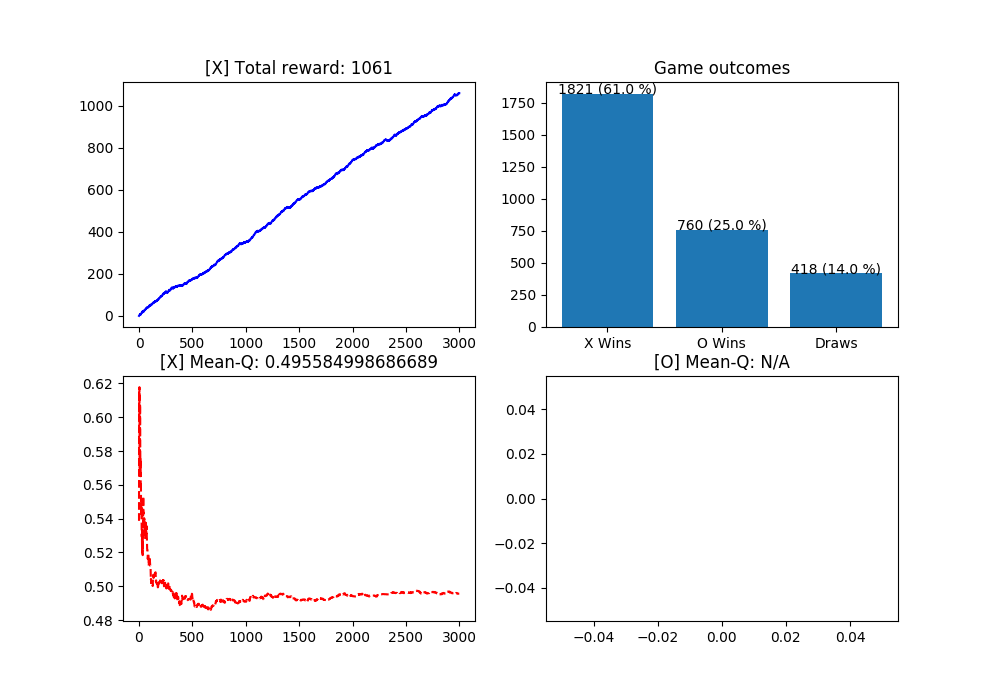
\includegraphics[width=0.7\linewidth]{imgs/q_learning/analysis/no_batch/lr/lr_0.png}
	\caption{Badania działania Q-learningu dla parametru $learning\_rate = 0$.}
\end{figure}

\begin{figure}[H]
	\centering
	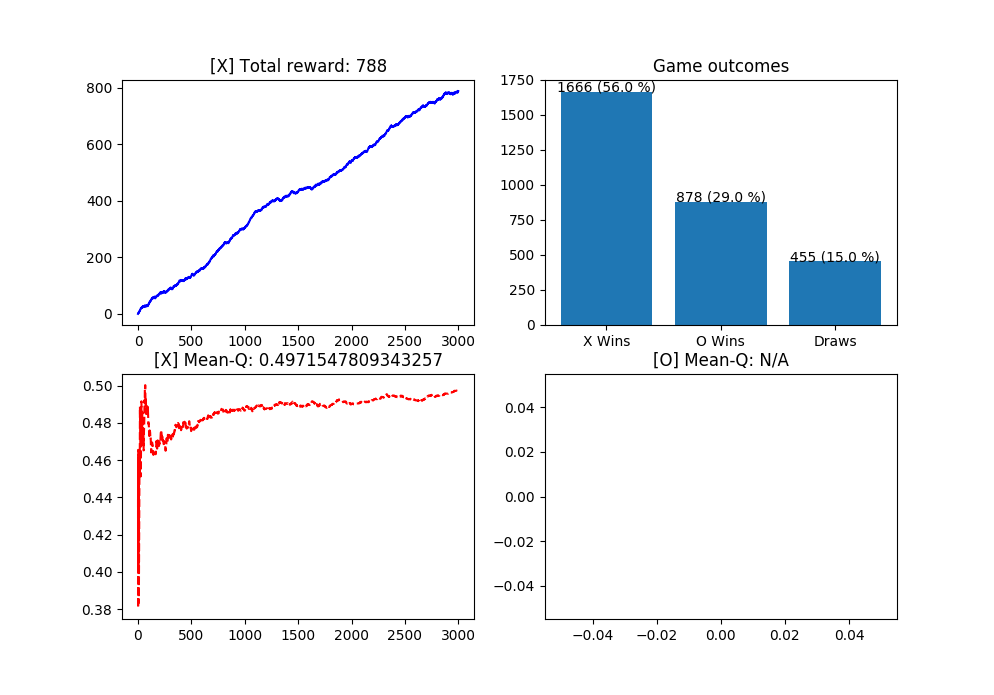
\includegraphics[width=0.7\linewidth]{imgs/q_learning/analysis/no_batch/lr/lr_0001}
	\caption{Badania działania Q-learningu dla parametru $learning\_rate = 0.001$.}
\end{figure}

\begin{figure}[H]
	\centering
	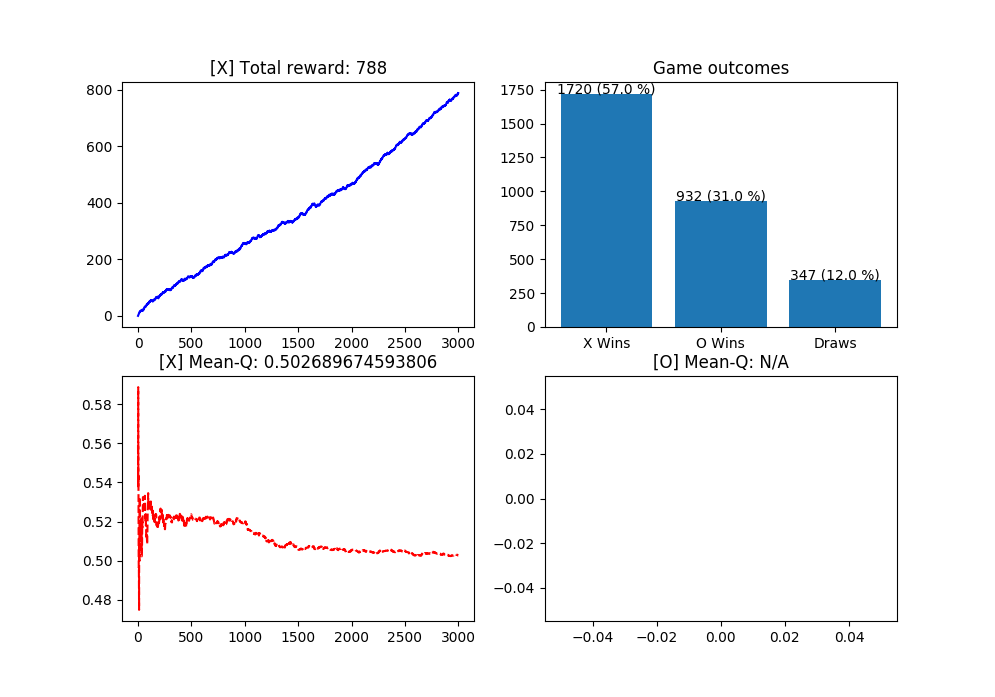
\includegraphics[width=0.7\linewidth]{imgs/q_learning/analysis/no_batch/lr/lr_001}
	\caption{Badania działania Q-learningu dla parametru $learning\_rate = 0.01$.}
\end{figure}

\begin{figure}[H]
	\centering
	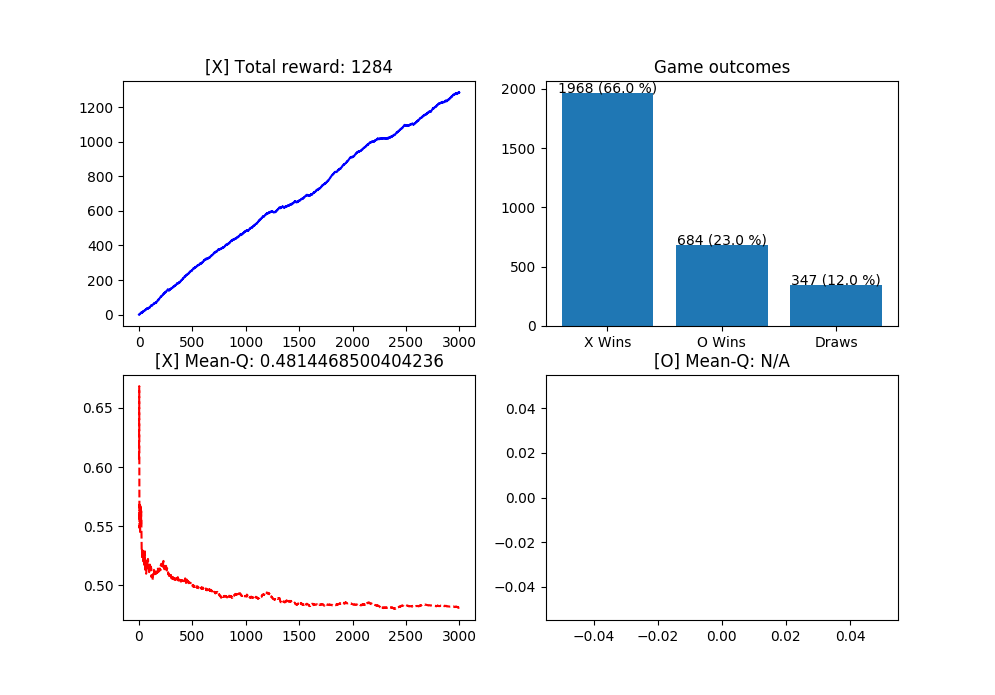
\includegraphics[width=0.7\linewidth]{imgs/q_learning/analysis/no_batch/lr/lr_01}
	\caption{Badania działania Q-learningu dla parametru $learning\_rate = 0.1$.}
\end{figure}

\begin{figure}[H]
	\centering
	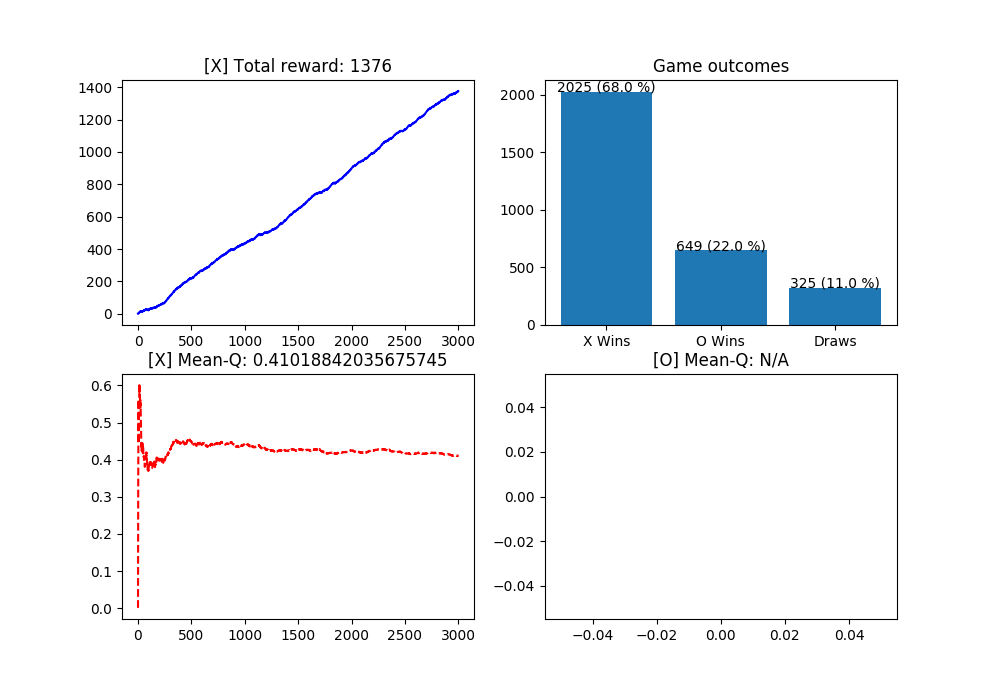
\includegraphics[width=0.7\linewidth]{imgs/q_learning/analysis/no_batch/lr/lr_1}
	\caption{Badania działania Q-learningu dla parametru $learning\_rate = 1$.}
\end{figure}

\pagebreak

\textbf{Discount factor}
%df
\begin{figure}[H]
	\centering
	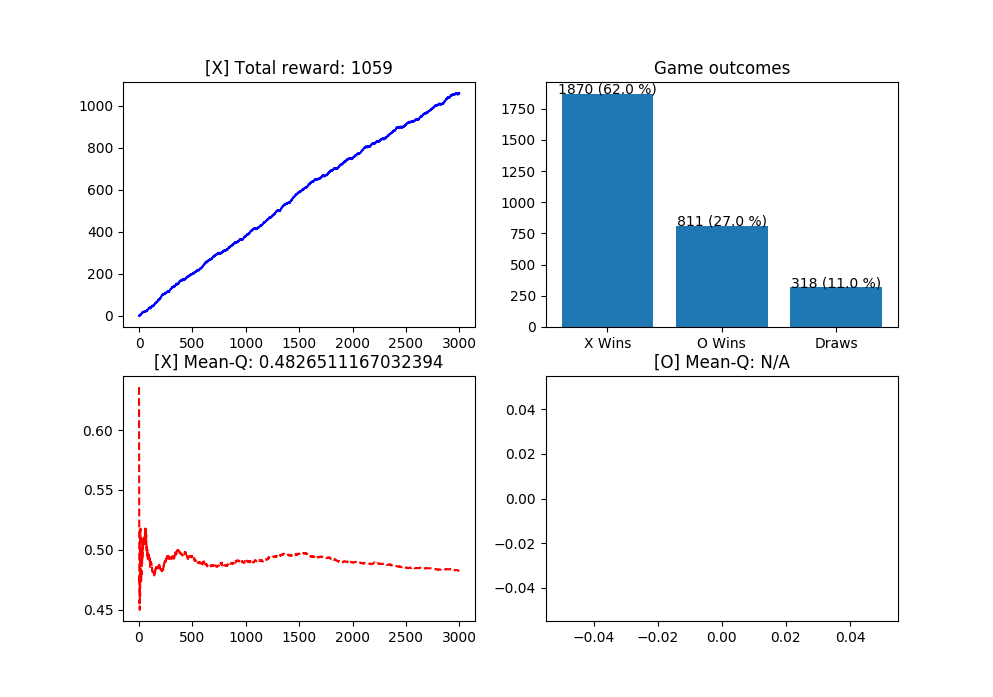
\includegraphics[width=0.7\linewidth]{imgs/q_learning/analysis/no_batch/df/df_0}
	\caption{Badania działania Q-learningu dla parametru $discount\_factor = 0$.}
\end{figure}

\begin{figure}[H]
	\centering
	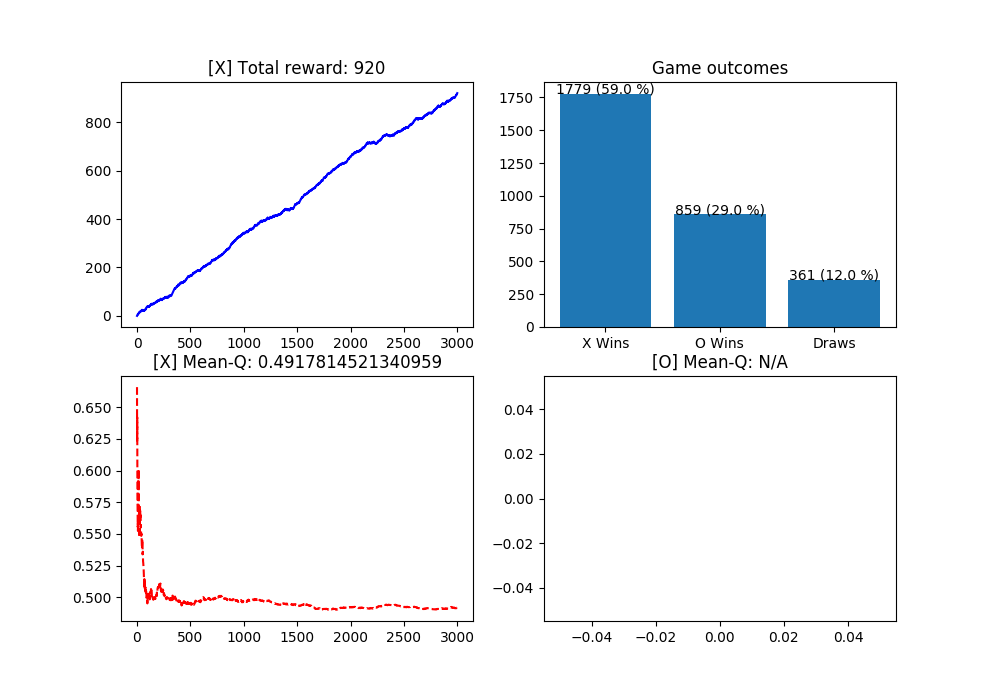
\includegraphics[width=0.7\linewidth]{imgs/q_learning/analysis/no_batch/df/df_025}
	\caption{Badania działania Q-learningu dla parametru $discount\_factor = 0.25$.}
\end{figure}

\begin{figure}[H]
	\centering
	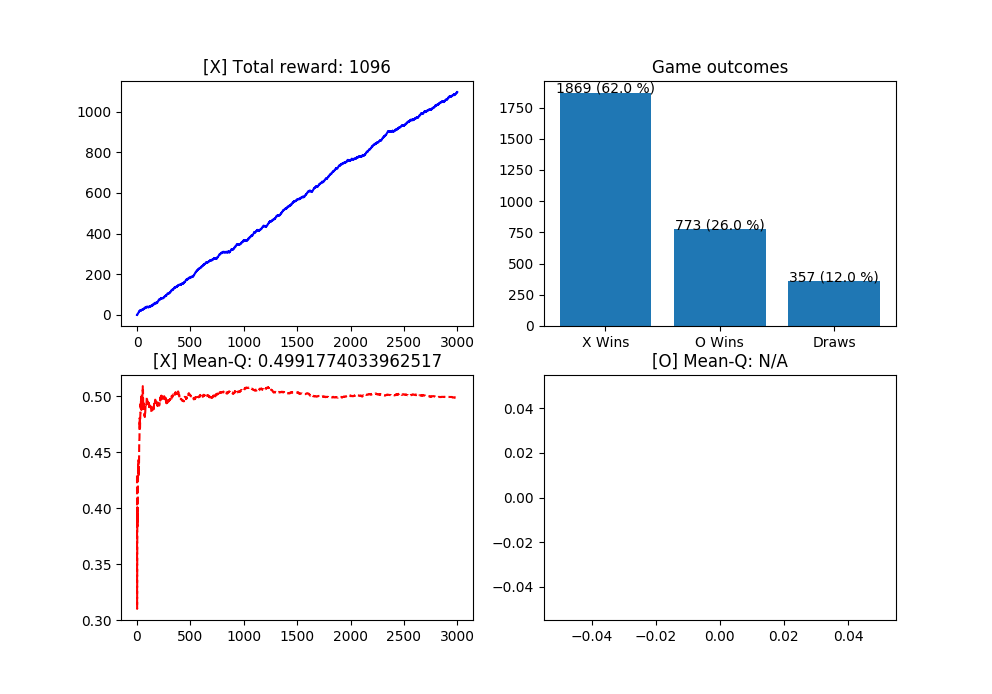
\includegraphics[width=0.7\linewidth]{imgs/q_learning/analysis/no_batch/df/df_05}
	\caption{Badania działania Q-learningu dla parametru $discount\_factor = 0.5$.}
\end{figure}

\begin{figure}[H]
	\centering
	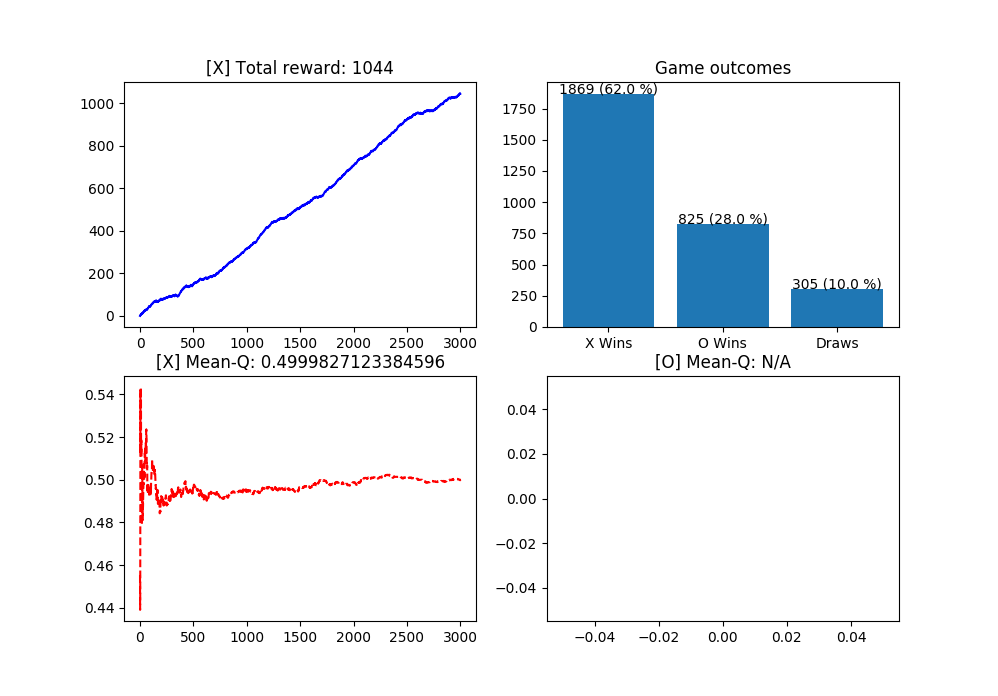
\includegraphics[width=0.7\linewidth]{imgs/q_learning/analysis/no_batch/df/df_075}
	\caption{Badania działania Q-learningu dla parametru $discount\_factor = 0.75$.}
\end{figure}

\begin{figure}[H]
	\centering
	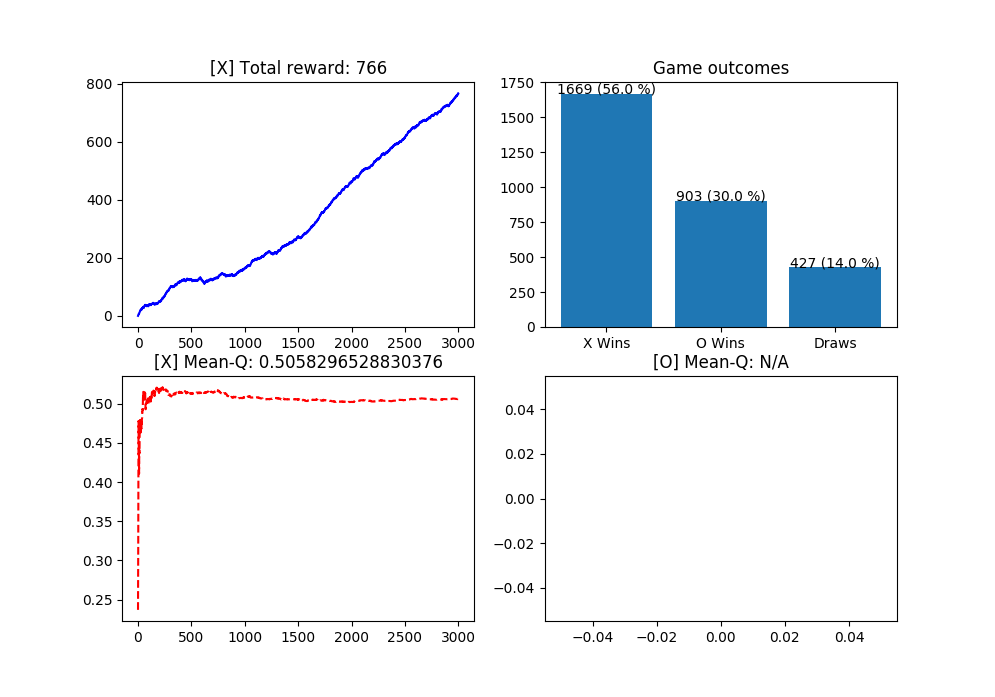
\includegraphics[width=0.7\linewidth]{imgs/q_learning/analysis/no_batch/df/df_1}
	\caption{Badania działania Q-learningu dla parametru $discount\_factor = 1$.}
\end{figure}

\pagebreak

\textbf{Epsilon}
%eps
\begin{figure}[H]
	\centering
	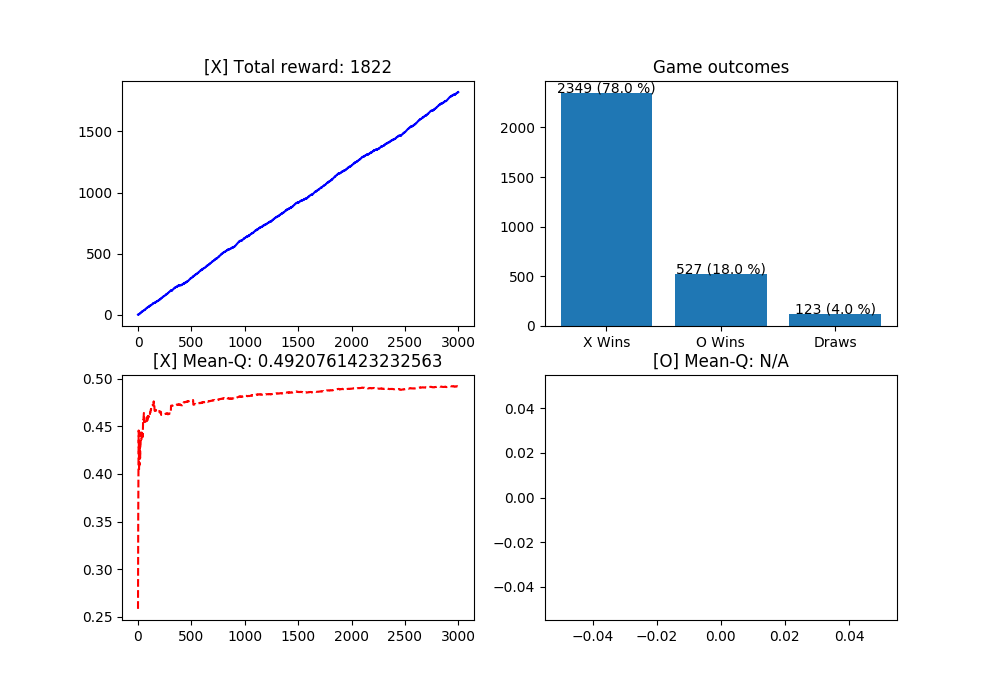
\includegraphics[width=0.7\linewidth]{imgs/q_learning/analysis/no_batch/eps/eps_0}
	\caption{Badania działania Q-learningu dla parametru $epsilon = 0$.}
\end{figure}

\begin{figure}[H]
	\centering
	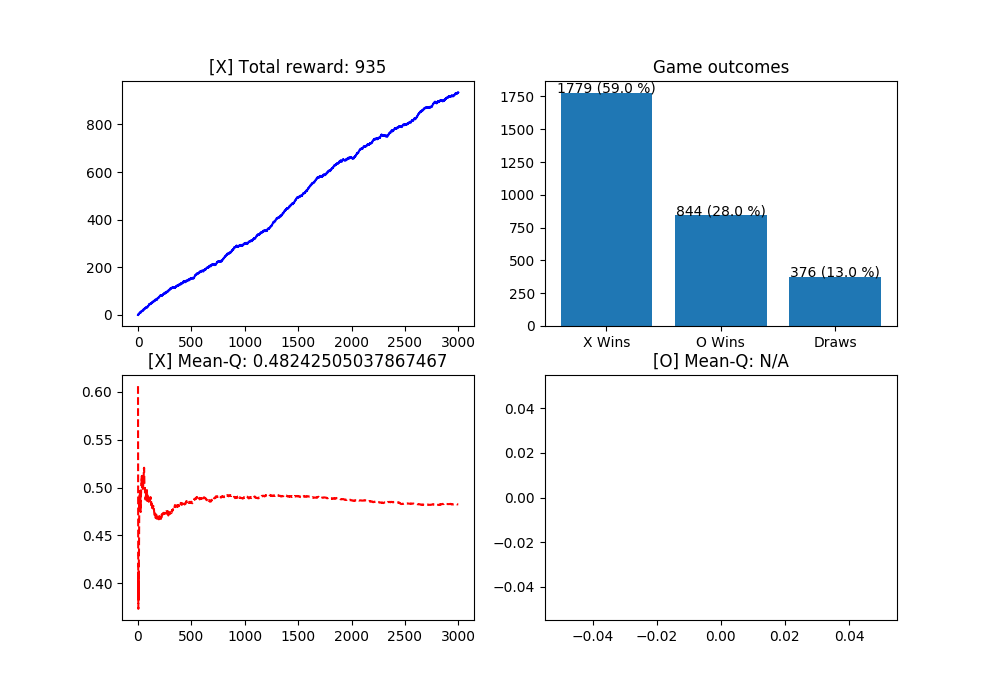
\includegraphics[width=0.7\linewidth]{imgs/q_learning/analysis/no_batch/eps/eps_02}
	\caption{Badania działania Q-learningu dla parametru $epsilon = 0.2$.}
\end{figure}

\begin{figure}[H]
	\centering
	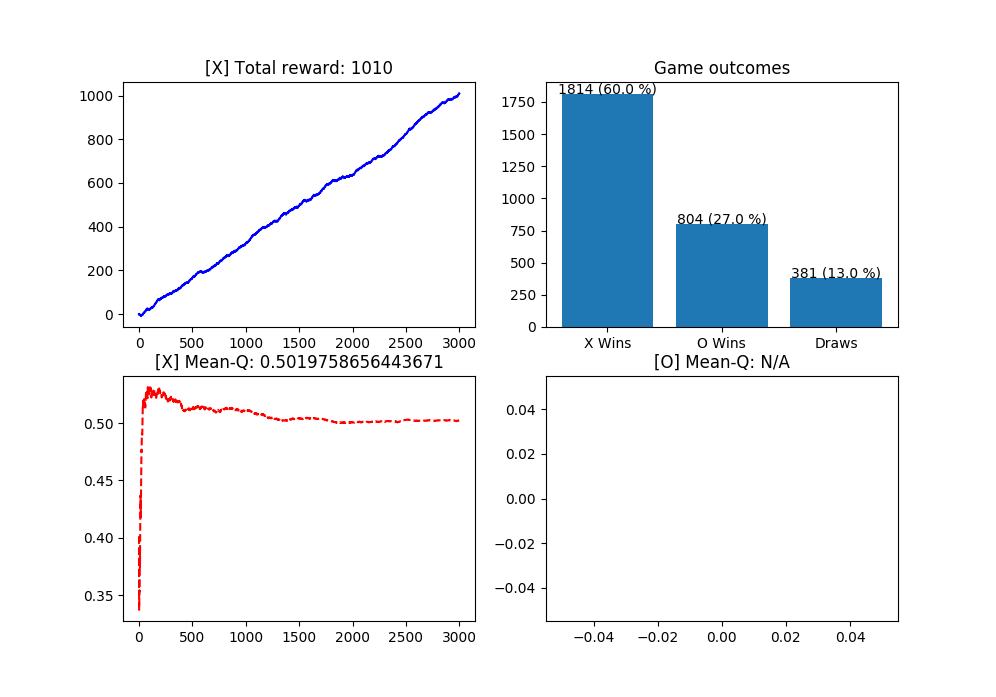
\includegraphics[width=0.7\linewidth]{imgs/q_learning/analysis/no_batch/eps/eps_05}
	\caption{Badania działania Q-learningu dla parametru $epsilon = 0.5$.}
\end{figure}

\begin{figure}[H]
	\centering
	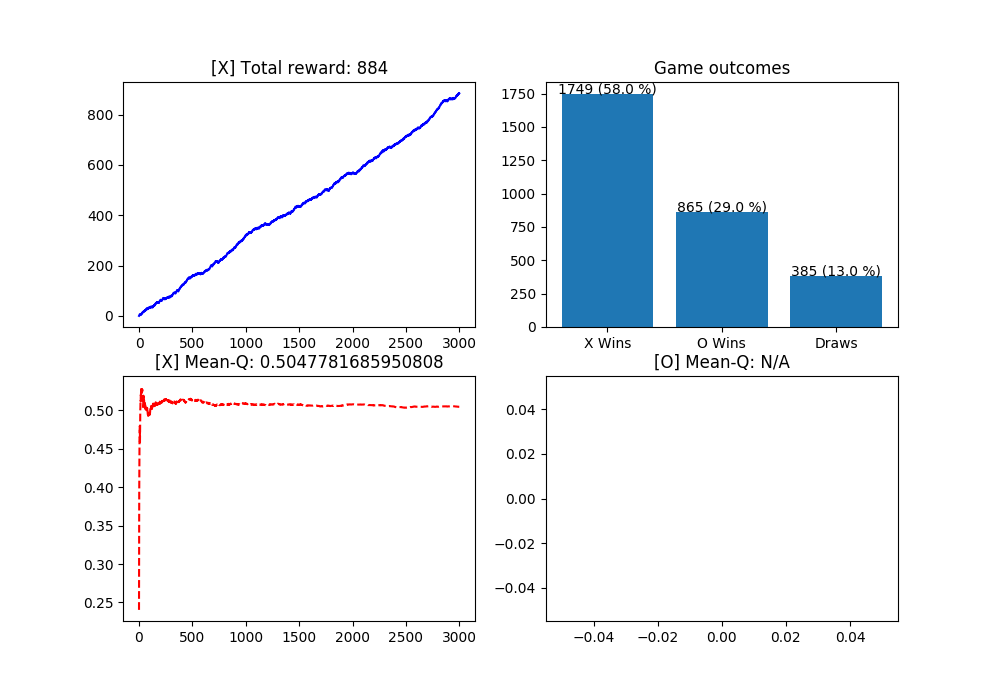
\includegraphics[width=0.7\linewidth]{imgs/q_learning/analysis/no_batch/eps/eps_1}
	\caption{Badania działania Q-learningu dla parametru $epsilon = 1$.}
\end{figure}

\pagebreak

\subsubsection{Batch mode}
% batch mode

\textbf{Learning rate}
% lr
\begin{figure}[H]
	\centering
	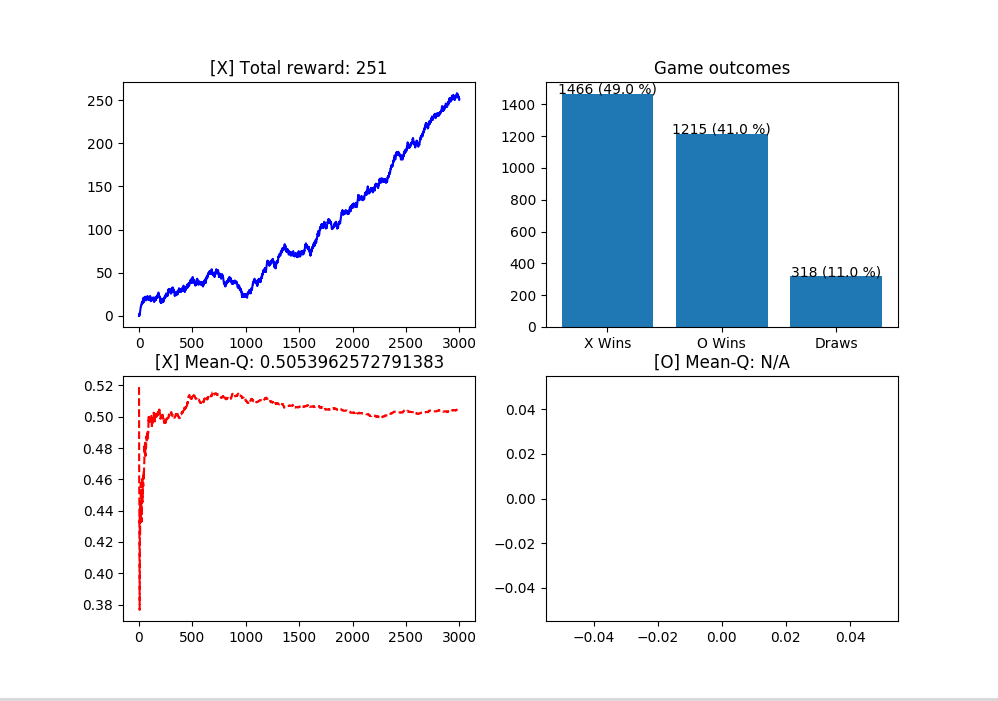
\includegraphics[width=0.7\linewidth]{imgs/q_learning/analysis/batch/lr/lr_0.png}
	\caption{Badania działania Q-learningu dla parametru $learning\_rate = 0$.}
\end{figure}

\begin{figure}[H]
	\centering
	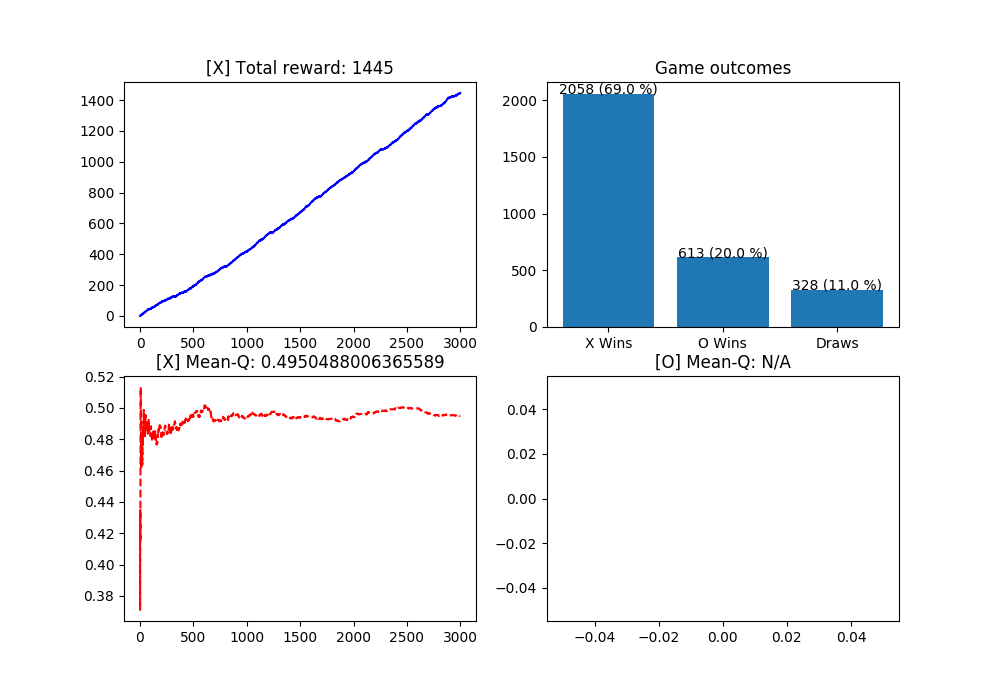
\includegraphics[width=0.7\linewidth]{imgs/q_learning/analysis/batch/lr/lr_0001}
	\caption{Badania działania Q-learningu dla parametru $learning\_rate = 0.001$.}
\end{figure}

\begin{figure}[H]
	\centering
	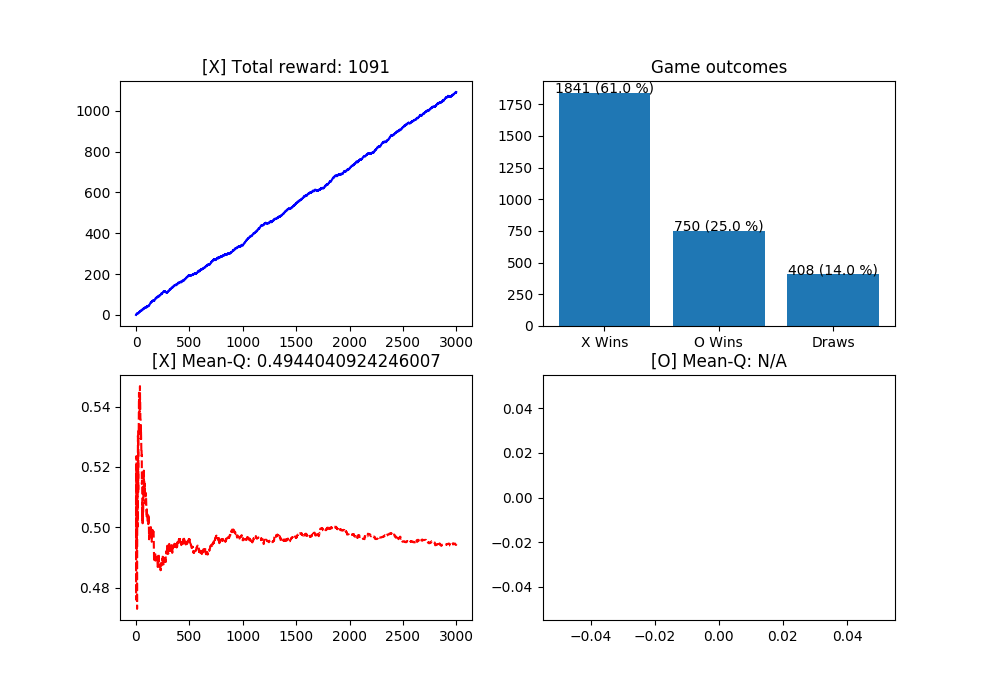
\includegraphics[width=0.7\linewidth]{imgs/q_learning/analysis/batch/lr/lr_001}
	\caption{Badania działania Q-learningu dla parametru $learning\_rate = 0.01$.}
\end{figure}

\begin{figure}[H]
	\centering
	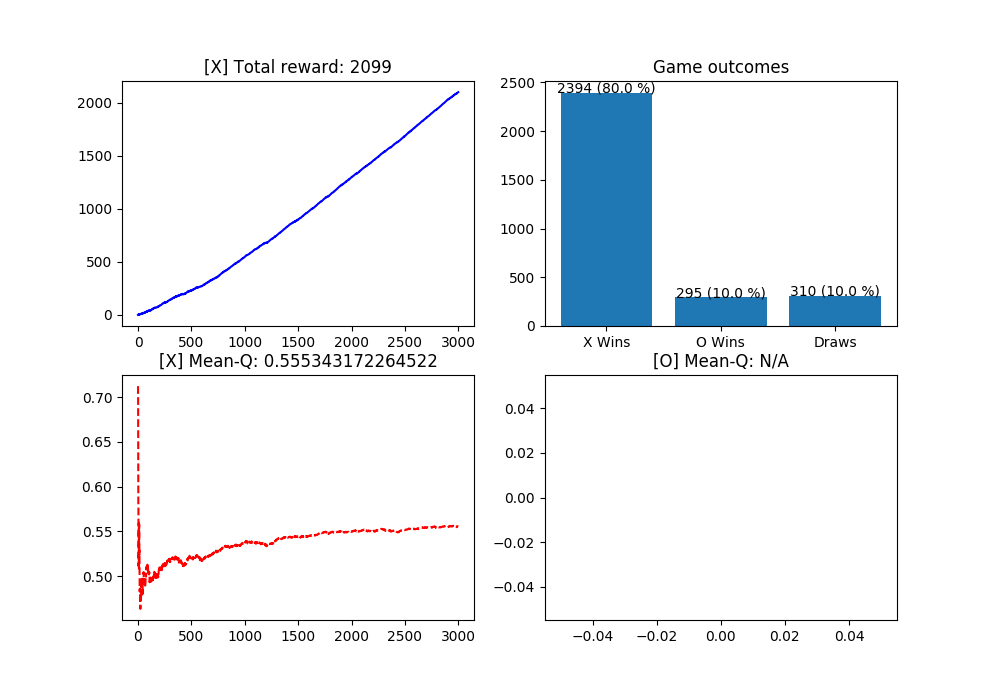
\includegraphics[width=0.7\linewidth]{imgs/q_learning/analysis/batch/lr/lr_01}
	\caption{Badania działania Q-learningu dla parametru $learning\_rate = 0.1$.}
\end{figure}

\begin{figure}[H]
	\centering
	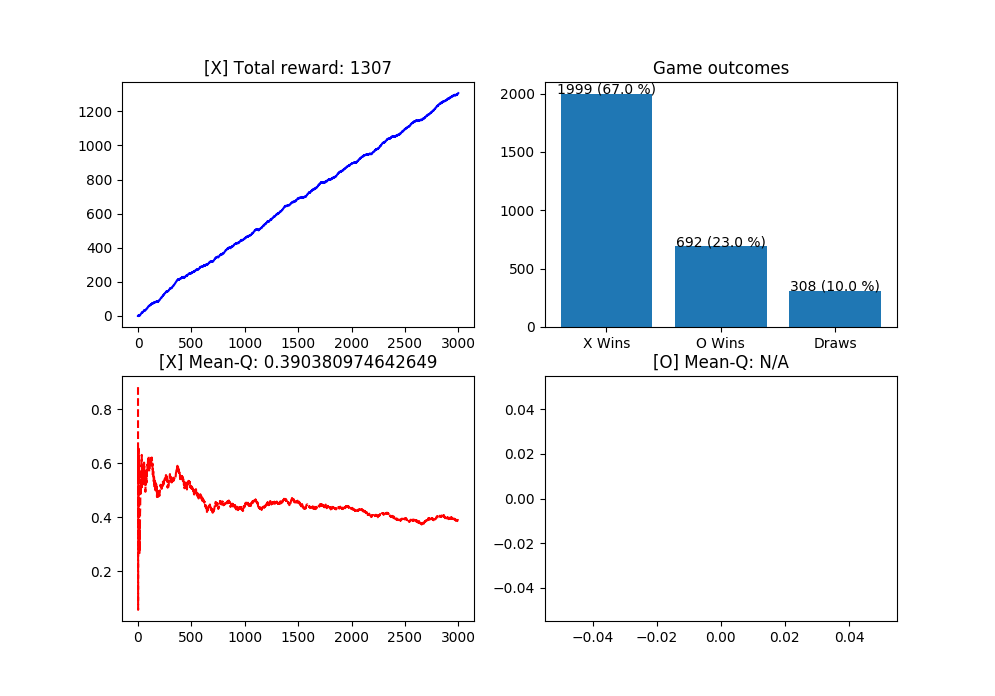
\includegraphics[width=0.7\linewidth]{imgs/q_learning/analysis/batch/lr/lr_1}
	\caption{Badania działania Q-learningu dla parametru $learning\_rate = 1$.}
\end{figure}

\pagebreak

\textbf{Discount factor}
%df
\begin{figure}[H]
	\centering
	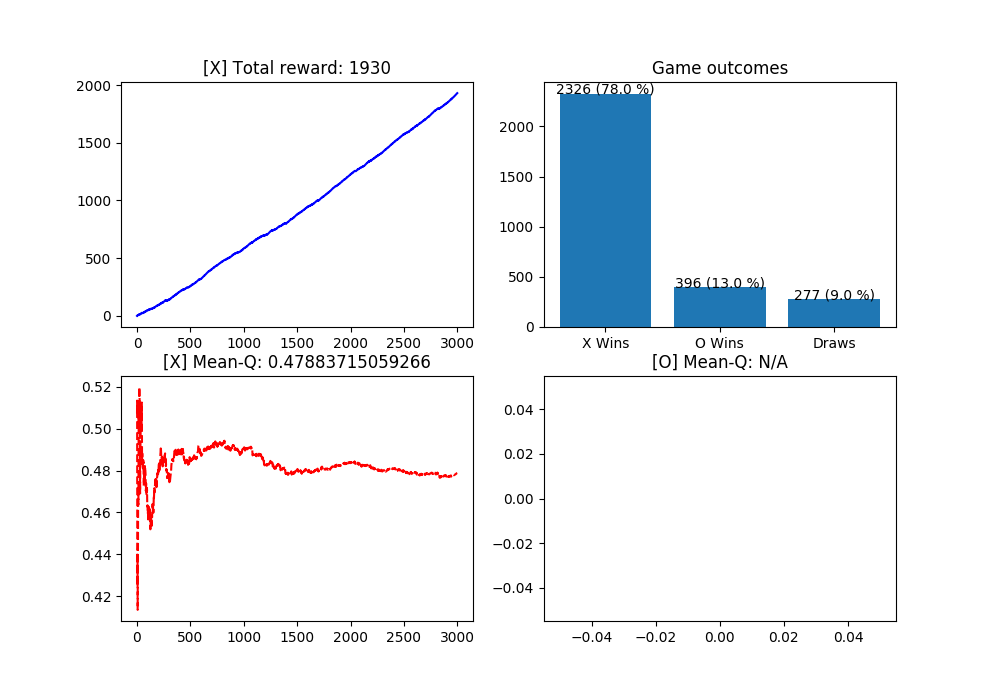
\includegraphics[width=0.7\linewidth]{imgs/q_learning/analysis/batch/df/df_0}
	\caption{Badania działania Q-learningu dla parametru $discount\_factor = 0$.}
\end{figure}

\begin{figure}[H]
	\centering
	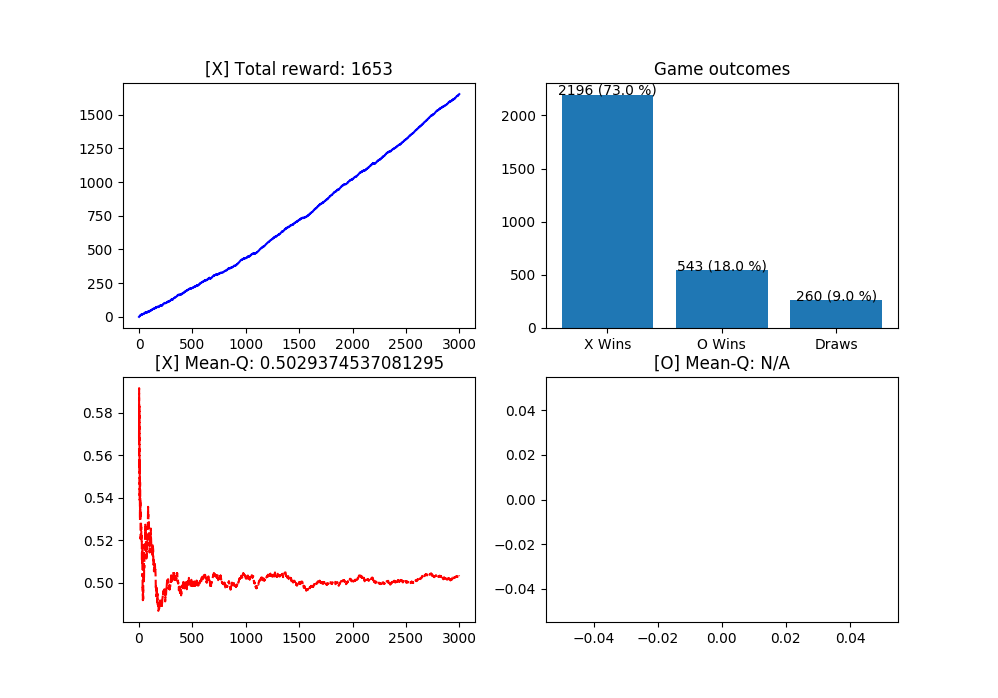
\includegraphics[width=0.7\linewidth]{imgs/q_learning/analysis/batch/df/df_025}
	\caption{Badania działania Q-learningu dla parametru $discount\_factor = 0.25$.}
\end{figure}

\begin{figure}[H]
	\centering
	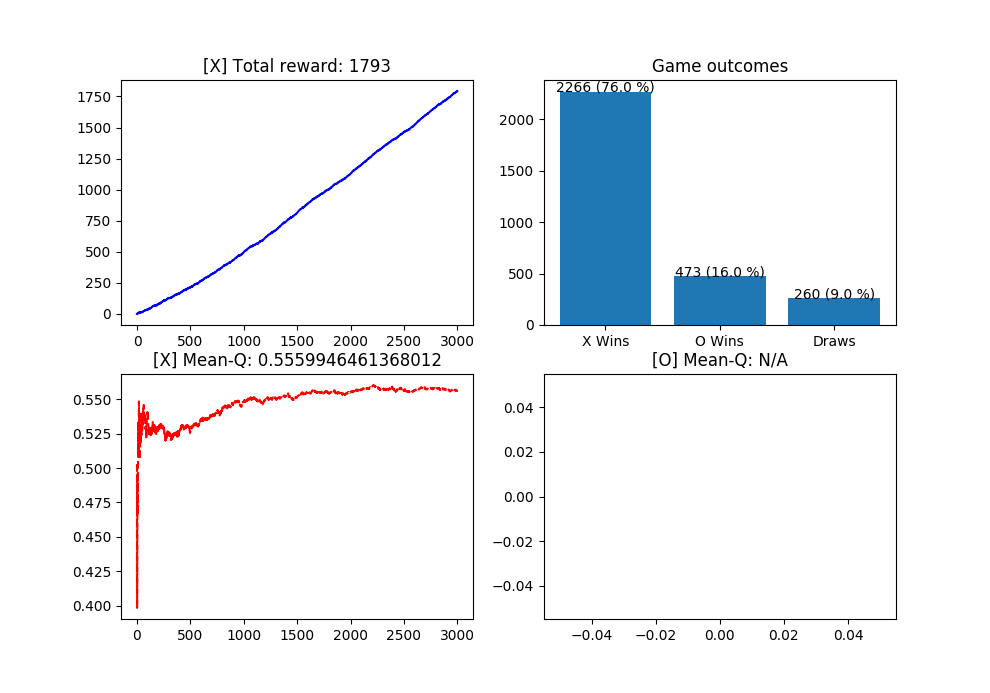
\includegraphics[width=0.7\linewidth]{imgs/q_learning/analysis/batch/df/df_05}
	\caption{Badania działania Q-learningu dla parametru $discount\_factor = 0.5$.}
\end{figure}

\begin{figure}[H]
	\centering
	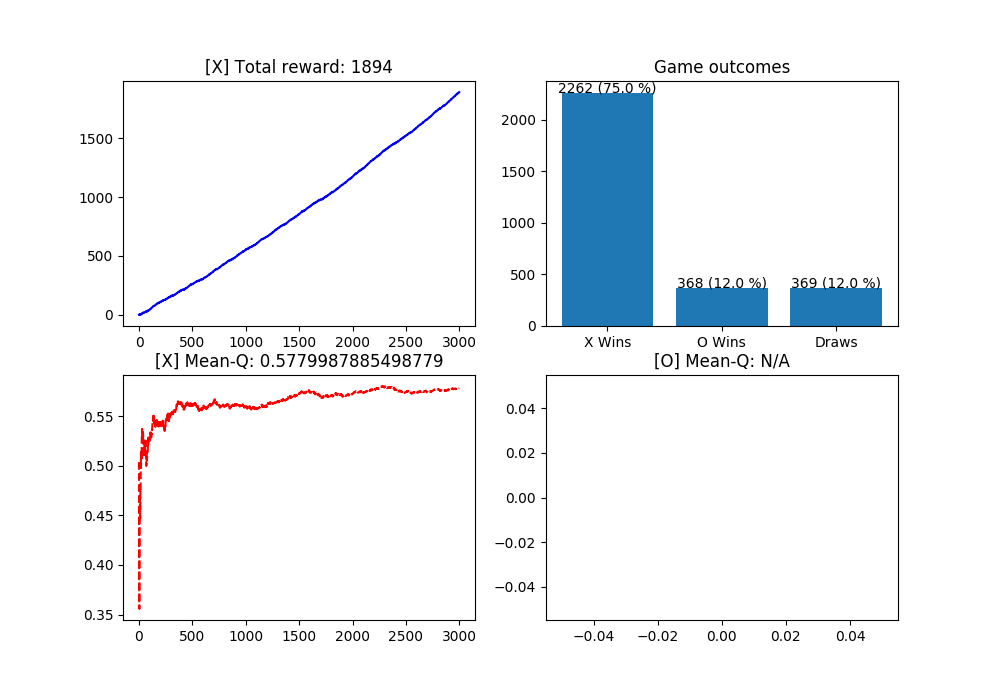
\includegraphics[width=0.7\linewidth]{imgs/q_learning/analysis/batch/df/df_075}
	\caption{Badania działania Q-learningu dla parametru $discount\_factor = 0.75$.}
\end{figure}

\begin{figure}[H]
	\centering
	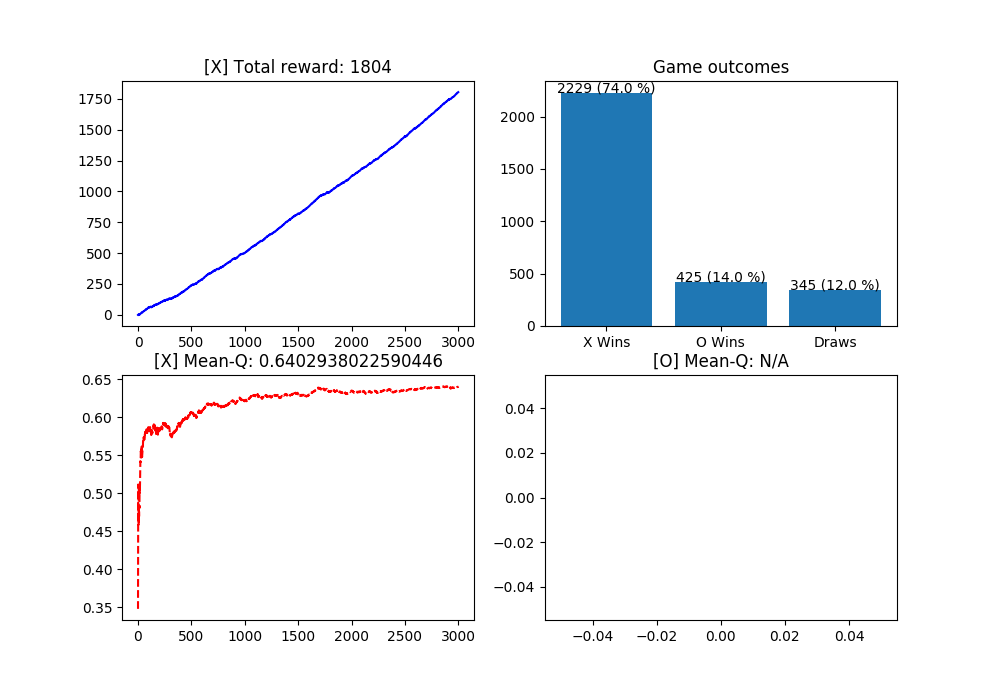
\includegraphics[width=0.7\linewidth]{imgs/q_learning/analysis/batch/df/df_1}
	\caption{Badania działania Q-learningu dla parametru $discount\_factor = 1$.}
\end{figure}

\pagebreak

\textbf{Epsilon}
%eps
\begin{figure}[H]
	\centering
	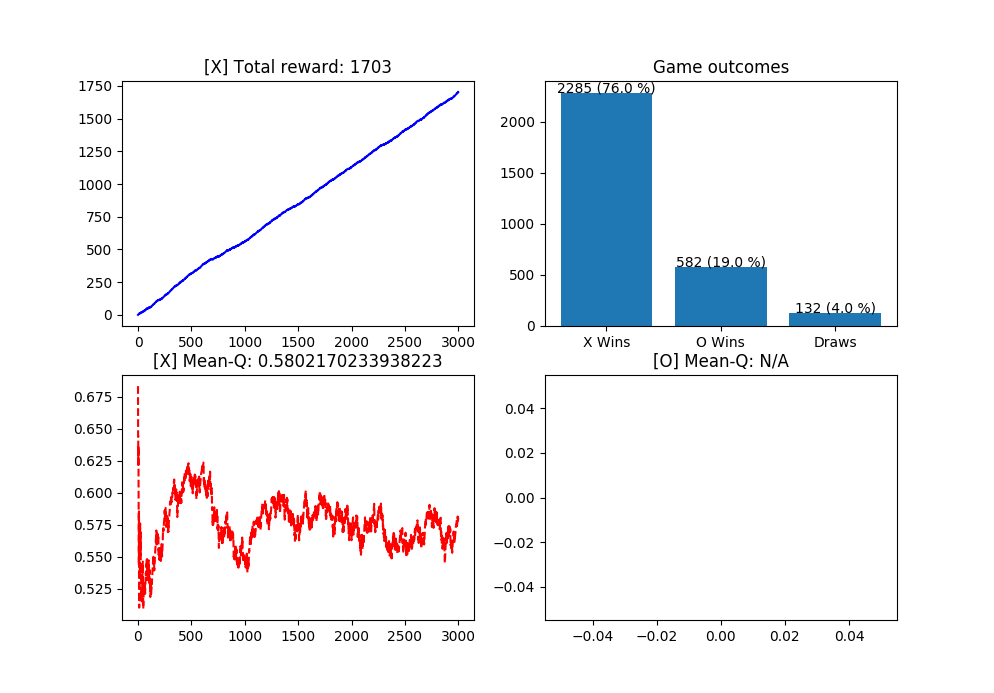
\includegraphics[width=0.7\linewidth]{imgs/q_learning/analysis/batch/eps/eps_0}
	\caption{Badania działania Q-learningu dla parametru $epsilon = 0$.}
\end{figure}

\begin{figure}[H]
	\centering
	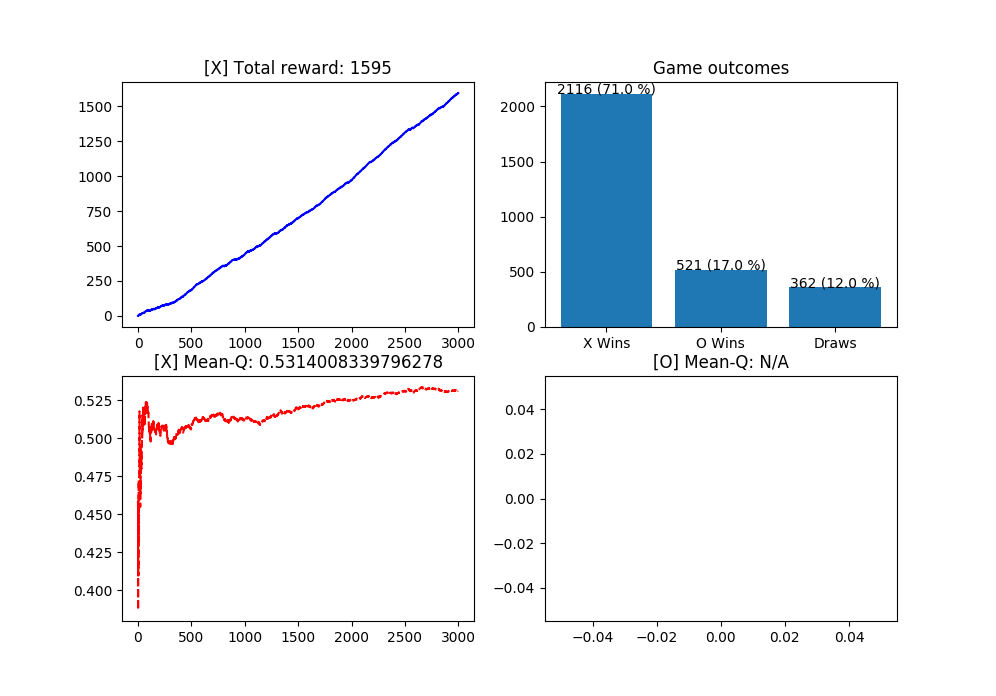
\includegraphics[width=0.7\linewidth]{imgs/q_learning/analysis/batch/eps/eps_02}
	\caption{Badania działania Q-learningu dla parametru $epsilon = 0.2$.}
\end{figure}

\begin{figure}[H]
	\centering
	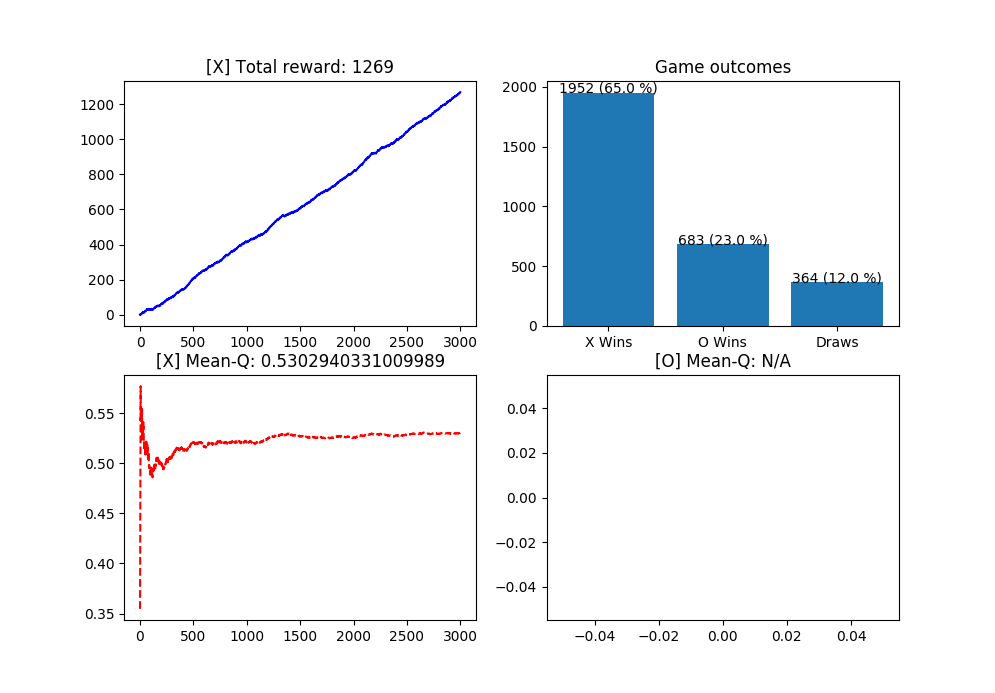
\includegraphics[width=0.7\linewidth]{imgs/q_learning/analysis/batch/eps/eps_05}
	\caption{Badania działania Q-learningu dla parametru $epsilon = 0.5$.}
\end{figure}

\begin{figure}[H]
	\centering
	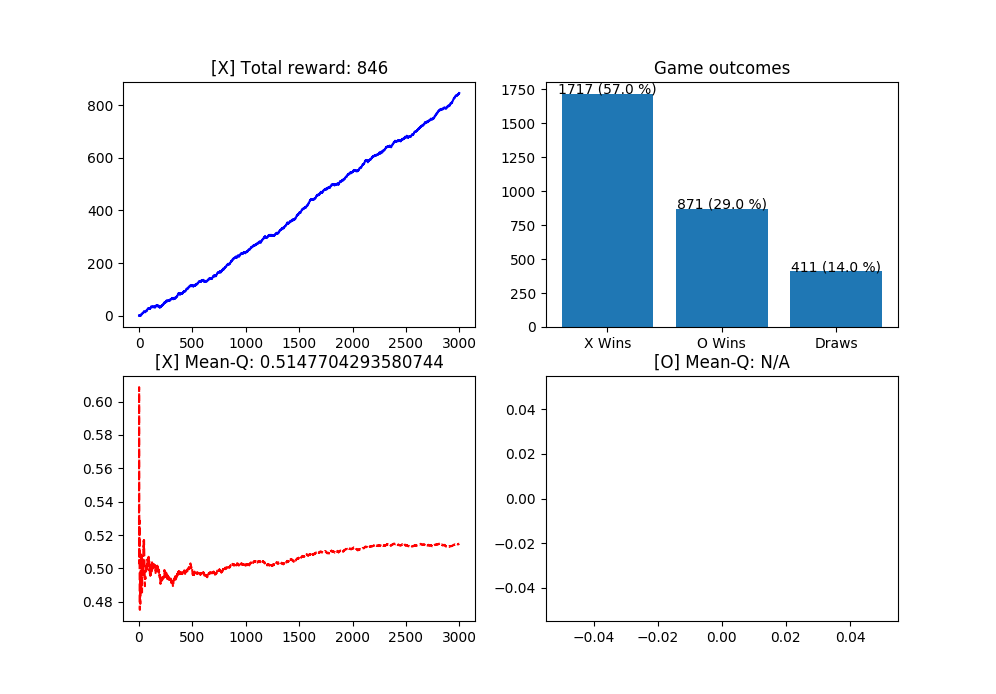
\includegraphics[width=0.7\linewidth]{imgs/q_learning/analysis/batch/eps/eps_1}
	\caption{Badania działania Q-learningu dla parametru $epsilon = 1$.}
\end{figure}

\subsection{Typy agentów}

\subsubsection{Q-learning - Random}

\begin{figure}[H]
	\centering
	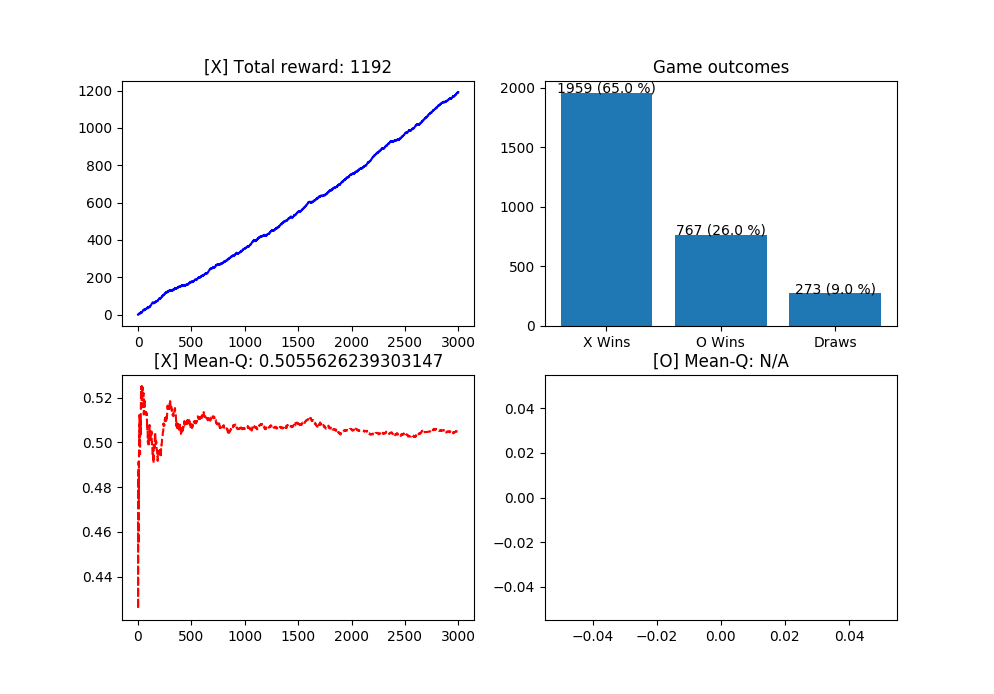
\includegraphics[width=0.7\linewidth]{imgs/q_learning/vs/q-r}
	\caption{Rozgrywka Q-learning oraz Random z użyciem domyślnych parametrów.}
\end{figure}

\begin{figure}[H]
	\centering
	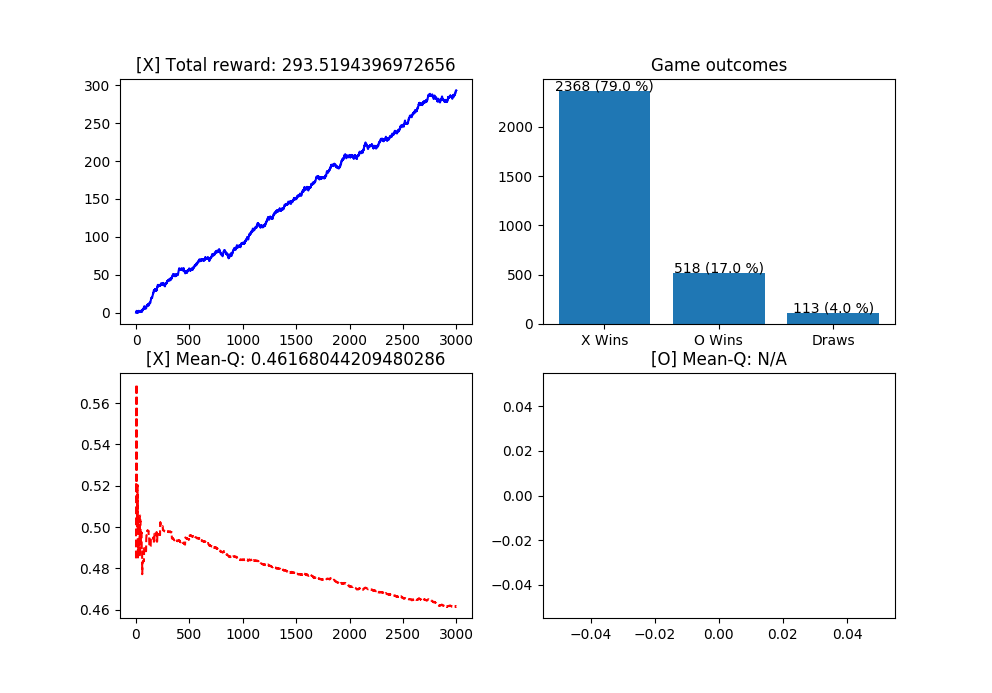
\includegraphics[width=0.7\linewidth]{imgs/q_learning/vs/q-r-supervised}
	\caption{Rozgrywka Q-learning oraz Random z użyciem uczenia nadzorowanego.}
\end{figure}

\subsubsection{Q-learning - Q-learning}

\begin{figure}[H]
	\centering
	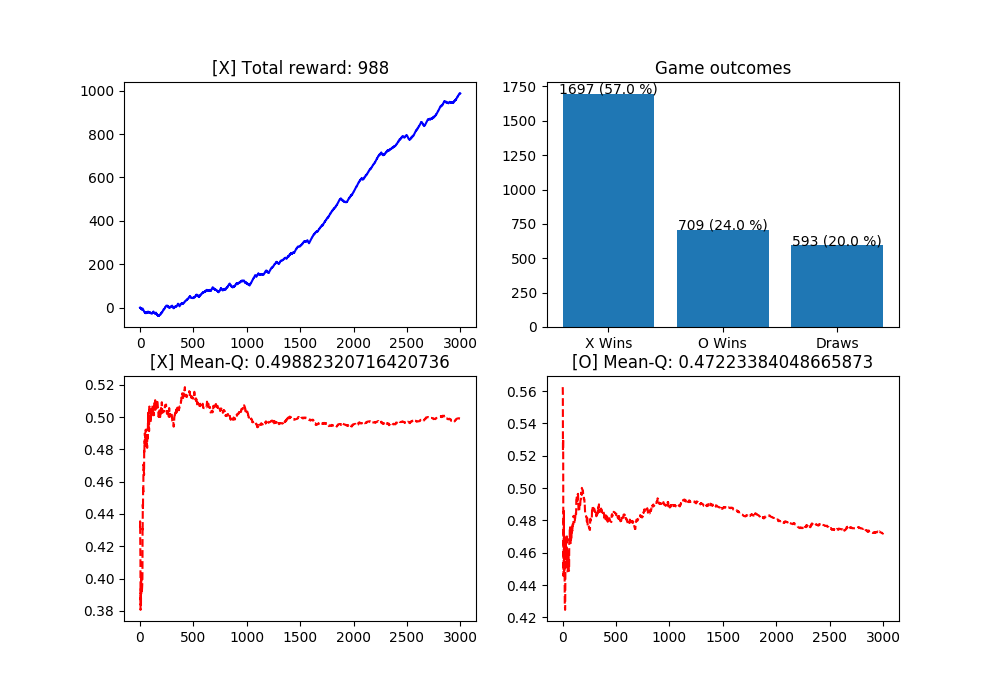
\includegraphics[width=0.7\linewidth]{imgs/q_learning/vs/q-q}
	\caption{Rozgrywka Q-learning oraz Q-learning z użyciem domyślnych parametrów.}
\end{figure}

\begin{figure}[H]
	\centering
	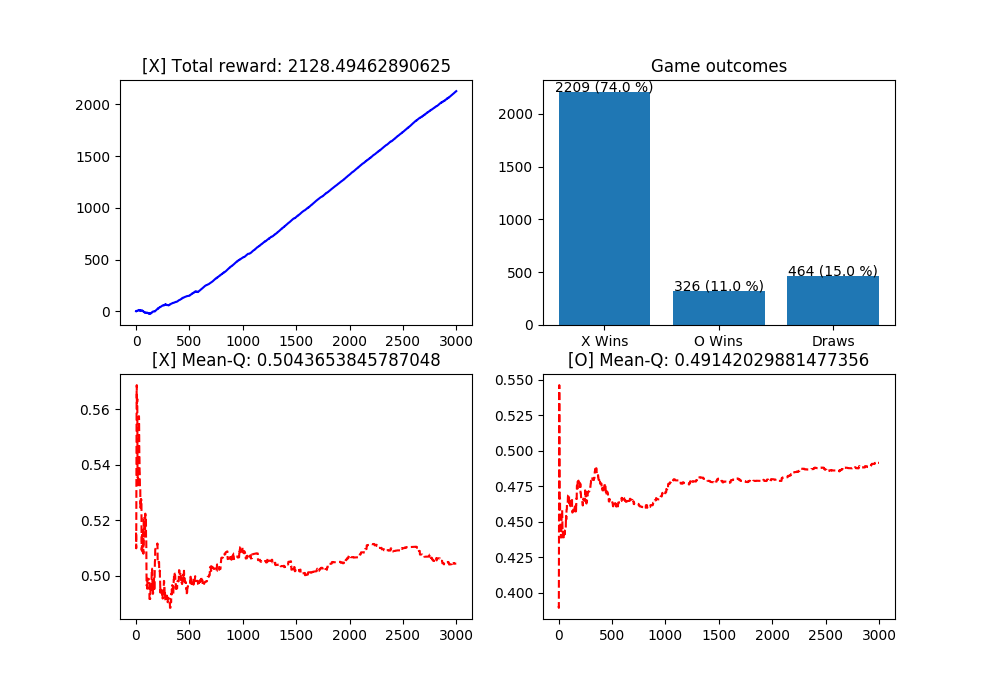
\includegraphics[width=0.7\linewidth]{imgs/q_learning/vs/q-q-supervised}
	\caption{Rozgrywka Q-learning oraz Q-learning z użyciem uczenia nadzorowanego.}
\end{figure}

\subsubsection{Ciekawostki}

\begin{figure}[H]
	\centering
	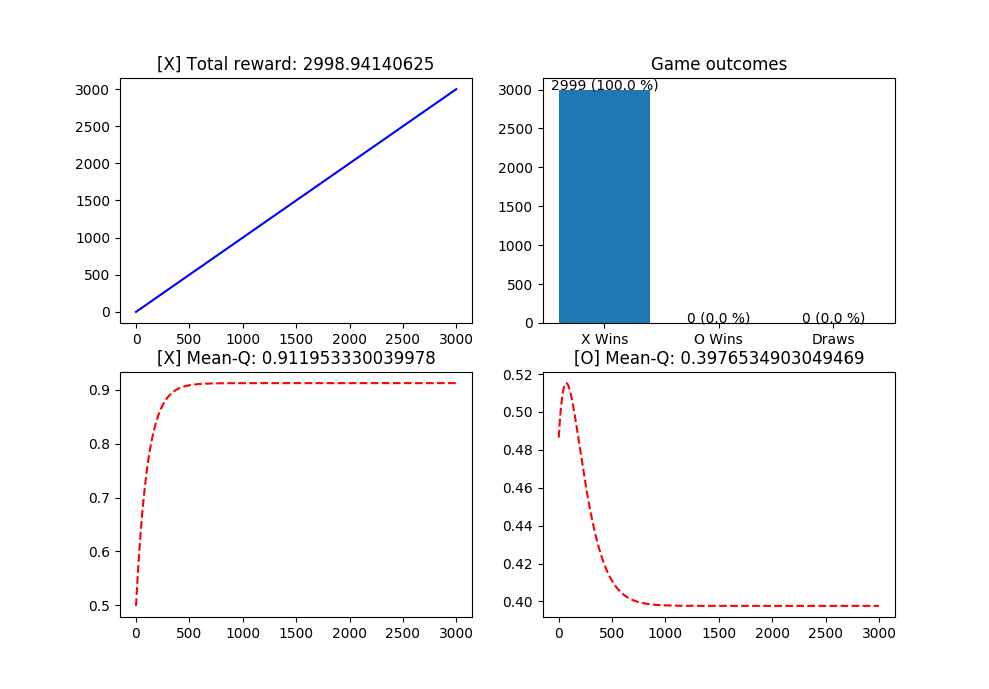
\includegraphics[width=0.7\linewidth]{imgs/q_learning/vs/q-q-miracle}
	\caption{Rozgrywka Q-learning oraz Q-learning z użyciem uczenia nadzorowanego, dla parametru $epsilon = 0$.}
\end{figure}

\pagebreak